\section{Acquisition}
\label{section:acquisition}

An acquisition is a collection of sensor data (laser scans and images) collected by the sensors in the scanner. Both sensors sample only a small subset of the whole environment: the laser scans only have points from a planar region of the space and cameras are limited by their focal length. To overcome this limitation, both sensors are moved to different poses in space to cover a wider space. In this case, the cause of movement of the sensors is the movement of the joints of the PTU. 

\subsection{Movement Programming}

To program the motion of the PTU joints, a list of waypoints in pan and tilt are defined and the joints move from waypoint to waypoint. The waypoints are defined in a grid in the joint-space and the movement between waypoints is the one that defines the shortest path possible and most of the movement is done in pan. So, each acquisition is parameterized with the following parameters: the range (minimum and maximum angle) of pan/tilt, the speed of each join and the number of waypoints in pan/tilt. An example of this parameterization can be seen in \cref{figure:joint-movement}.

Once the movement of the scanner was defined, the next step is to define when to record the laser scans and the images, according to it. Because of the nature of both sensors, it was established that laser scans are captured continuously during the pan movement between the waypoints and images are captured at every waypoint.

\begin{figure}[h]

    \centering
    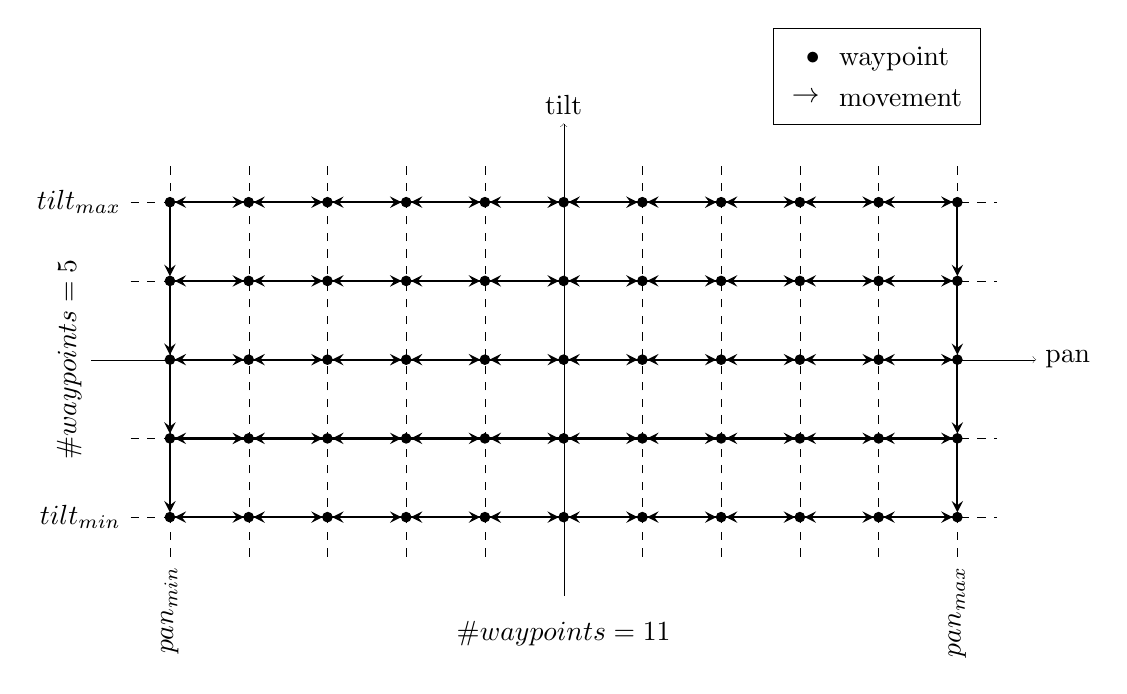
\begin{tikzpicture}

        \draw[->, ultra thin] (-6, 0) -- (6, 0) node[right] {pan};
        \draw[->, ultra thin] (0, -3) -- (0, 3) node[above] {tilt};

        \draw[step=1, ultra thin, dashed] (-5.5, -2.5) grid (5.5, 2.5);

        \foreach \x in {-5,...,5}
            \foreach \y in {-2,...,2}
                \draw[fill=black] (\x, \y) circle (0.06);
        
        \foreach \x in {-5,...,4}
            \foreach \y in {-2,...,2}
                \ifthenelse{\isodd{\y}}{
                    \draw[stealth-, shorten <=0.06cm, thick] (\x, \y) -- (\x+1, \y);  
                }{
                    \draw[-stealth, shorten >=0.06cm, thick] (\x, \y) -- (\x+1, \y);
                };

        \foreach \y in {2,...,-1}
            \ifthenelse{\isodd{\y}}{
                \draw[-stealth, shorten >=0.06cm, thick] (-5, \y) -- (-5, \y - 1);
            }{
                \draw[-stealth, shorten >=0.06cm, thick] (5, \y) -- (5, \y - 1);
            };

        
        \node[anchor=east] at (-5.5, -2) {$tilt_{min}$};
        \node[anchor=east] at (-5.5, 2) {$tilt_{max}$};
        \node[anchor=south, rotate=90] at (-6, 0) {$\#waypoints = 5$};

        \node[anchor=east, rotate=90] at (-5, -2.5) {$pan_{min}$};
        \node[anchor=east, rotate=90] at (5, -2.5) {$pan_{max}$};
        \node[anchor=north] at (0, -3.2) {$\#waypoints=11$};
            
        \matrix[draw, above left, xshift=-1.5cm, yshift=-0.5cm] at (current bounding box.north east) {
            \node[label=right:waypoint] {$\bullet$}; \\
            \node[label=right:movement] {$\rightarrow$}; \\
        };

    \end{tikzpicture}

    \caption{Waypoints and movements in the pan/tilt joint space.}

\label{figure:joint-movement}
\end{figure}


\subsection{Parameterization Considerations}

This methodology has the following implications:

\begin{itemize}
        
    \item The pan and tilt range is only limited by the PTU capabilities, but it beneficial to use the maximum range possible, in order to get as much data as it is possible, even if some data is redundant. In this work, the mobile scanner have a laser configuration such that the interpolation if different tilt angles is almost exclusively redundant data. However, this improves the final reconstruction by increasing the density of the point cloud.
                    
    \item The number of laser scans recorded is going to depend on the pan speed and the frequency of scanning of the 2D laser scanner. So, it is expected that a laser scanner with a lower scanning frequency to require a slower speed compared to a faster one, to get the same results. 
                        
    \item The camera used in this work did not have stabilization so, to get sharp images, a complete immobilization was required in each waypoint. This was achieved by setting a time between the stop of all joints and the capture of the image by the camera. In this work, a time of \SI{1.5}{\second} was enough.
                        
    \item The waypoints' angle increment has to be enough so that part of the previous image appear in the next image, so that every observable part of the scene is seen at least once. This depends heavily on the focal point of the camera: the bigger the focal point, the least area it captures and more waypoints are required.
                    
\end{itemize}

\subsection{Default Parameters}
\label{section:acquisition-default-parameters}

\subsection{Acquisition node}
\label{section:acquisition-node}


To implement this functionality, a ROS node was developed according to the previously defined specifications. This node, called \emph{single\_acquisition\_node} is present in the \emph{lemonbot\_acquisition} package and the way is implemented is the following: the PTU movement is controlled by it and the selected messages are republished into a new topic. For convenience, all the acquisition topics are republished into the \emph{/acquisition} namespace. So, during an acquisition, two topics can be found, each one corresponding to each sensor, inside this namespace: the laser scans are in \emph{/acquisition/laserscans} and the images are in \emph{/acquisition/images}. This idea of republishing all the important messages greatly improved the acquisition organization, so all the topics that were required were also republished into this namespace. This topics were the \emph{/acquisition/camera\_info}, containing the intrinsic parameters of the camera, and \emph{/acquisition/tf} and \emph{/acquisition/tf\_static}, containing all the transformations of the robot.

Now, data from this topics need to be saved permanently, so this was done using a ROS tool called \emph{rosbag}, that saves all the data from a predefined set of topics into a binary file called a \emph{bag} file. This was a easy and powerful solution, because it allows the acquisition to be reproduced again, by republishing all the messages back into the system. To save a set of topics, a node called \emph{record} from the \emph{rosbag} package is run with the list of topics that required to be recorded into disk. In this case, the required topics are all the topics inside the \emph{/acquisition} namespace.

To streamline the acquisition process, all this components (the acquisition node, the topic republisher nodes and the rosbag record node) can be all launched through a \emph{launch file}. A set of all the parameters required for each acquisition can be override over the default parameters shown in \cref{section:acquisition-default-parameters}. Therefore, running an acquisition just requires a single command:

\begin{verbatim}
roslaunch lemonbot_acquisition single_acquisition.launch \
    pan_min:=-90 pan_max:=90 pan_vel:=10 pan_nsteps:=25 \
    tilt_min:=-15 tilt_max:=15 tilt_nsteps:=5
\end{verbatim}

In conclusion, running the previous command will run an acquisition and in the end, a bag file will be present, with the topics \emph{images}, \emph{laserscan}, \emph{camera\_info}, \emph{tf} and \emph{tf\_static}, therefore all the information relevant for the reconstruction.

To have a better insight in the bag file, a tool called \emph{rosbag info} can be used. All the details about when the calibration took place, how long it took as well as how many messages it contains are printed. An example of this information is:

\begin{figure}
    
    \begin{Verbatim}
path:        acquisition_2018-09-07-16-01-46.bag
version:     2.0
duration:    4:53s (293s)
start:       Sep 07 2018 16:01:47.11 (1536332507.11)
end:         Sep 07 2018 16:06:40.96 (1536332800.96)
size:        87.0 MB
messages:    6690
compression: none [16/16 chunks]
types:       sensor_msgs/CameraInfo [c9a58c1b0b154e0e6da7578cb991d214]
                sensor_msgs/Image      [060021388200f6f0f447d0fcd9c64743]
                sensor_msgs/LaserScan  [90c7ef2dc6895d81024acba2ac42f369]
                tf2_msgs/TFMessage     [94810edda583a504dfda3829e70d7eec]
topics:      camera_info    953 msgs    : sensor_msgs/CameraInfo
                images          10 msgs    : sensor_msgs/Image     
                laserscan     2788 msgs    : sensor_msgs/LaserScan 
                tf            2938 msgs    : tf2_msgs/TFMessage    
                tf_static        1 msg     : tf2_msgs/TFMessage
    \end{Verbatim}

    \caption{Example of a recorded bag file info}
    \label{figure:bag-file-example}
\end{figure}

\subsection{Data Serialization}
 
Despite it's potentiality, bag files are not the best way to store the acquisition data for the reconstruction pipeline. There are some limitations of bag files in this application. The most noticeable is that the full transformation graph is stored, while in fact only the transformations between the start and end frame of the PTU are needed, as well as the transformations between the PTU mount link and each one of the sensors, which are static. Also, this transformation messages are not synchronized with the laser scans and image messages, which means an interpolation has to be performed each time the data is read. Another drawback is that bag files stores messages in it's own format, which hinder reading and inspecting the data, which can be helpful to check if an acquisition was successful. For example, the images are serialized into a ROS message, instead of being in a file with a known format, like \emph{JPG}, which would allow for easier access and inspection.

To solve this issues, a preprocessing of the bag files was performed, to convert and extract all the important information into well known and useful formats. Each laser scan was stored in a \emph{AVRO} file row that contains the timestamp (when it was taken), the minimum and maximum angle (aperture of the laser scan), the minimum and maximum ranges that the laser can capture, the transformation of the ptu and the list of all the measured ranges. An example of such row is show in \cref{figure:laserscan-row}, obtained using the \emph{avro cat} command. Each image was stored in a separate \emph{JPEG} file and it's timestamp and transformation was stored in a row, again in a \emph{AVRO} file. The parameters inherent to the acquisition, such as the name of the bag, the extrinsic and intrinsic calibration of the camera used and the extrinsic calibration of the laser was stored in a \emph{YAML} file. The transformations in both the images and laser scans are stored as vector for translation and quaternion for rotation.

\begin{figure}
    
    \begin{Verbatim}[frame=single]
{
    "ranges" : [ ... ],
    "limits" : {
        "min" : 0.100000001490116,
        "max" : 29
    },
    "timestamp" : 1536174204611117487,
    "angles" : {
        "min" : -2.35619449615479,
        "max" : 2.35619449615479
    },
    "transform" : {
        "rotation" : [ ... ],
        "translation" : [ ... ]
    }
}
    \end{Verbatim}

    \caption{Example of laser scan row}
\label{figure:laserscan-row}
\end{figure}

\begin{figure}

    \begin{Verbatim}[frame=single]
bag: acquisition_2018-09-05-20-02-46.bag
camera:
    extrinsic:
    translation: [ ... ]
    rotation: [ ... ]
    intrinsic:
    principal_point: [ ... ]
    height: 1448
    focal_lenghts: [ ... ]
    width: 1928
    distortion_coef: [ ... ]
    distortion_model: plumb_bob
laser:
    extrinsic:
    translation: [ ... ]
    rotation: [ ... ]
    limits:
        max: 29
        min: 0.1
    angles:
        max: 2.356194
        min: -2.356194
    \end{Verbatim}

    \caption{Example of the parameters YAML file}

\end{figure}

